\textbf{COLUNI 2026 -- Questão 04}\par\medskip \textbf{Leia o texto I para responder às questões 1 a 4:}

\begin{center}\textbf{A MORTE E O REI}\end{center}

Noite, ainda não. Mas as nuvens tão escuras, que era como se fosse. E nesse escuro pesado, envolta num manto, a Morte galopava seu cavalo negro em direção ao castelo. Os cascos incandescentes incendiavam a grama. Desfaziam-se as pedras em centelhas.

Diante da muralha, sequer chamou ou apeou para bater ao portão. O manto estalava ao vento. O cavalo escarvava com a pata. Ela esperava.

E logo os pesados batentes se abriram num estridor de ferragens. E a Temível foi levada à presença do Rei.

- Vim buscar-vos, Senhor - disse sem rodeios.

- Não contestaria chamado tão definitivo, sem boa razão - respondeu o monarca, com igual precisão, com igual precisão. - Peço-lhe, porém que não partamos já. Realiza-se amanhã um torneio nos jardins do castelo. E tenho certeza de que sua presença dará outro valor à disputa.

Um instante bastou para a Morte avaliar o pedido. E concordar. Afinal, um dia a menos pouco pesaria na eternidade. Mas muito pesaria os que ela havia de levar.

Recolheu-se, pois, esperando o amanhecer.

Ainda no escuro, agitava-se o castelo preparando o torneio. Cavaleiros chegavam de longe. Tendas eram armadas nos jardins. Fogueiras ardiam nas oficinas dos armeiros. Quando o sol veio, farfalharam as sedas, os galhardetes, as folhas das árvores, e um mesmo brilho metálico saltou dos olhares, das couraças, das joias das damas. Em breve, soaram as trombetas, os cavalos partiram a galope. E o sangue floresceu sobre a grama.

À noite, a Sussurrada novamente dirigiu-se ao Rei.

- Senhor, em minha morada, esperam por nós.

- Na minha também, Senhora, somos esperados - respondeu o Rei, com voz dura. - Informantes acabaram de me revelar que um grupo de conspiradores está pronto para levantar suas armas contra mim.

E depois de ter dado tempo para que ela avaliasse suas palavras, acrescentou em tom mais baixo, quase envolvente: - Os que se escondem nas sombras precisarão da sua assistência.

Amplas são as sombras, pensou a Morte, calculando a sua parte. E mais uma vez concordou em adiar a partida.

Ao entardecer do dia seguinte, um mancebo foi apunhalado num corredor escuro, um ministro foi passado ao fio da espada junto a uma coluna, enquanto no alto de uma escada uma dama tombava envenenada. Antes que o sol nascesse novamente, o carrasco decepou as outras cabeças que haviam ousado pensar contra o Rei.

- Senhor - disse a Intransponível depois de recolher a sua carga - já esperei mais do que devia. Mande selar o cavalo. E partamos.

- Esperou, é certo. Mas foi bem recompensada - respondeu o Rei. - Mandei selar o meu cavalo, como me pede. E partiremos. Porém não para seguir o seu caminho. Acabei de declarar guerra aos países do Leste. E preciso da sua presença ao meu lado, nos campos de batalha.

A Morte sabia, por antiga experiência, o quanto podia ceifar nesses campos. Sem discutir, emparelhou seu cavalo com o do Rei, e começou a longa marcha. À frente, muito trabalho a esperava.

Não era trabalho para um dia. Nem para dois. Dias e dias se passaram. Meses. Anos. Em que a Sombria parecia não ter descanso, cortando, quebrando, arrancando. E colhendo. Colhendo. Colhendo.

E porque ela havia colhido tanto, chegou um momento em que a guerra não tinha mais como prosseguir. E acabou.

À frente do exército dizimado, o Rei e a Morte regressaram ao castelo. E na sala, agora desguarnecida de seus cavaleiros, o Rei assinou o tratado de paz.

Molhada ainda a tinta, já a Insaciável se adiantava, lembrando ao Rei que uma outra viagem o aguardava.

- Irei sim, minha amiga - respondeu ele com voz gasta de tanto gritar ordens. - Mas amanhã. É tarde agora. E estou tão cansado. Deixe-me dormir só esta noite na minha cama.

E porque a Morte hesitava: - Seja generosa comigo que já lhe dei tanto - pediu.

Uma noite, pensou a Invencível, não faria diferença. E ela também merecia um pouco de descanso. Como na noite da sua chegada, agora tão distante, recolheu-se.

Silêncio no castelo. Só sonhos percorriam os corredores. Mas no seu quarto, o Rei estava desperto. A hora havia chegado. Levantou-se, envolveu-se num manto, agarrou o castiçal com a vela acesa e, abrindo a pequena porta encoberta por uma tapeçaria, meteu-se pela passagem secreta cuidando de não fazer qualquer ruído.

Desceu degraus, seguiu sobre o piso escorregadio entre paredes estreitas, desceu uma longa escada, avançou por uma espécie de interminável corredor, desceu outros degraus. E afinal, cabeça baixa para evitar as teias de aranha, puxou uma argola de ferro e abriu uma porta. Havia chegado às cavalariças.

A vela apagou-se num sopro de vento. Tateando, pegou uma sela, arreios, e com gestos rápidos encilhou um cavalo. Montou de um salto. Cravou as esporas, soltou as rédeas. E ei-lo lá fora, galopando na noite, afastando-se do castelo.

Galopava o cavalo. As nuvens abriram-se por um instante, a luz da Lua mordeu o pescoço do animal. Só então o Rei viu que o cavalo era mais negro que a escuridão. E que seus cascos incandescentes queimavam a grama ao passar, desfazendo as pedras em centelhas.

\begin{flushright}(COLASSANTI, Marina. A morte e o rei. In: \textbf{Com certeza tenho amor}. São Paulo: Global, 2009, p. 9-13.)\end{flushright}

A tirinha da série \textit{Malvados} e o conto \textit{A Morte e o Rei} apresentam a morte como personagem central, mas utilizam linguagens distintas. A comparação do uso dessas linguagens e de seus sentidos na representação da morte, nos textos I e II, está CORRETA em:

\textbf{Texto II}

% COLUNI-AUTO-FIGURES-BEGIN
\begin{figure}[htbp]
\centering
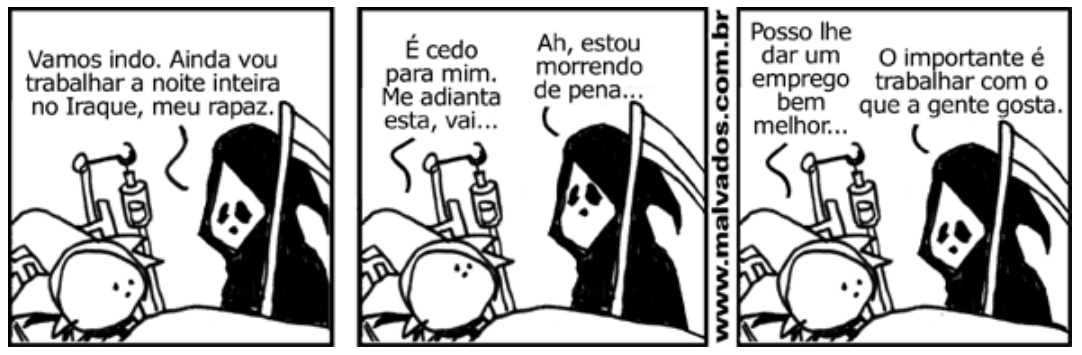
\includegraphics[width=0.85\linewidth]{static/simulados/coluni/figuras/2026/questao-04/figura-1.png}
\end{figure}
% COLUNI-AUTO-FIGURES-END
\begin{center}(Disponível em: https://www.malvados.com.br/index418.html. Acesso em: 20 ago. 2025)\end{center}
\begin{enumerate}
\item A tirinha utiliza imagens simples da morte com túnica preta e foice associadas a diálogos curtos, construindo um tom irônico para humanizar e banalizar a figura da morte como uma trabalhadora sobrecarregada; enquanto o conto recorre a descrições verbais detalhadas, criando uma atmosfera sombria em torno da morte, o que afirma a sua inevitabilidade.
\item A tirinha enfatiza, nos diálogos curtos e informais, que o trabalho de ceifar vidas é uma profissão desagradável, criando um efeito cômico; enquanto o conto recorre a estratégias narrativas em que o Rei, detentor de poder, solicita à Morte tempo para resolver suas pendências terrenas, revelando uma morte paciente e estrategista.
\item A tirinha apresenta imagens simples caracterizadas pelo contraste das cores preto e branco, contribuindo para a imagem fria e corruptível da morte; enquanto o conto explora as possibilidades plurissignificativas das palavras para materializar uma imagem da morte que se delineia a partir do imaginário de cada um.
\item A tirinha mobiliza o contraste das cores preto e branco, imagens simples e diálogos informais para aproximar a morte do cotidiano, criando uma atmosfera de leveza e aceitação; enquanto o conto lança mão de uma linguagem simples e objetiva, problematizando os principais impactos que a morte causa nos seres humanos, criando uma reflexão moral.
\end{enumerate}
